% $x_{\blop}$

In the following let $(H_\bullet,\partial_\bullet)$ be any homology theory.

\begin{lemma}
    Let $A \subseteq X$ be a retract. Then $H_\bullet(X) \cong H_\bullet(X,A) \oplus H_\bullet(A)$.
\end{lemma}

\begin{proof}
    Let $r \colon X \to A$ be a retraction and $i \colon A \to X$ the inclusion. Then $H_\bullet(r) \circ H_\bullet(i) = \mathrm{id}_{H_\bullet(A)}$, in particular $H_\bullet(i)$ is injective. Hence the long exact sequence for the pair $(X,A)$ breaks up into short split exact sequences
    \begin{center}
        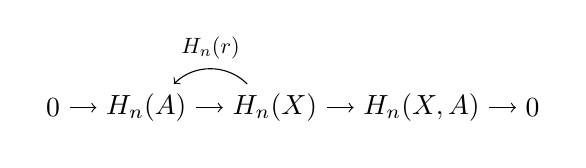
\begin{tikzpicture}
            \matrix[column sep = 10pt, row sep =15pt]
            {
                \node (zero1) {$0$}; &
                \node (hna) {$H_n(A)$}; &
                \node (hnx) {$H_n(X)$}; &
                \node (hnxa) {$H_n(X,A)$}; &
                \node (zero2) {$0$}; \\
            };

            \draw[->] (zero1.east) -- (hna.west);
            \draw[->] (hna.east) -- (hnx.west);
            \draw[->] (hnx.east) -- (hnxa.west);
            \draw[->] (hnxa.east) -- (zero2.west);
            \draw[->, bend right=45] ([xshift=-10pt]hnx.north) to node[above] {\scalebox{0.8}{$H_n(r)$}} ([xshift=10pt]hna.north);
        \end{tikzpicture}
    \end{center}
    and the splitting lemma yields the desired isomorphism.
\end{proof}

\begin{lemma}
    Let $A \subseteq X$ be a subspace, such that the inclusion $A \to X$ is a homotopy equivalence. Then $H_\bullet(X,A) = 0$.
\end{lemma}
\begin{proof}
    This follows from the long exact sequence for the pair $(X,A)$. Note that the inclusion $(A,A) \to (X,A)$ is not necessarily a homotopy equivalence.
\end{proof}

\begin{lemma}
    Let $A \subseteq X$ be a closed neighbourhood-deformation retract. Then the projection $X \to X/A$ induces a natural isomorphism $$H_\bullet(X,A) \to H_\bullet(X/A,\ast)$$.
\end{lemma}
\begin{proof}
    Applying excision in the push-out
    \begin{center}
        \commsquare{$A$}{$X$}{$\ast$}{$X/A$}{}{}{}{}
    \end{center}
    shows that the projection induces an isomorphism. Furthermore, any map $(X,A) \to (Y,B)$ descends to a map $X/A \to Y/B$ and naturality then just follows from functoriality. 

\end{proof}